\documentclass[a4paper,11pt]{article}
%Przydatne paczki:
\usepackage{amssymb}
\usepackage{amsthm}
\usepackage{amsmath}
\usepackage[colorinlistoftodos]{todonotes}
\usepackage[colorlinks=true, allcolors=blue]{hyperref}
%Definicja kodowania i języka:
\usepackage[polish]{babel}
\usepackage[MeX]{polski}
\usepackage[utf8]{inputenc}
\usepackage[T1]{fontenc}
%Paczki dodane w drodze pisania:
\usepackage{graphicx}
\usepackage{anysize}
\selectlanguage{polish}
\usepackage{tabularx}
\usepackage[export]{adjustbox}
\usepackage{listings}
\usepackage{float}
\usepackage{fancyhdr}
\usepackage{listing}

%Nagłówek:
\pagestyle{fancy}
\fancyhead{}
\fancyhead[L]{\small{\bfseries \thepage}}
\fancyfoot[L, C, R] {}
\fancyhead[C]{\small{\bfseries Dokumentacja projektu "Reflekto"}}
\renewcommand{\headrulewidth}{0.8pt}

%\marginsize{left}{right}{top}{bottom}
\marginsize{2.5cm}{2.5cm}{2.5cm}{2.5cm}
\lstdefinelanguage{C}{
	keywords={typeof, new, true, false, catch, function, return, null, catch, switch, var, if, in, while, do, else, case, break},
	keywordstyle=\color{blue}\bfseries,
	ndkeywords={class, export, boolean, throw, implements, import, this},
	ndkeywordstyle=\color{darkgray}\bfseries,
	identifierstyle=\color{black},
	sensitive=false,
	comment=[l]{//},
	morecomment=[s]{/*}{*/},
	commentstyle=\color{purple}\ttfamily,
	stringstyle=\color{red}\ttfamily,
	morestring=[b]',
	morestring=[b]"
}

\lstset{
	language=C,
	backgroundcolor=\color{lightgray},
	extendedchars=true,
	basicstyle=\footnotesize\ttfamily,
	showstringspaces=false,
	showspaces=false,
	numbers=left,
	numberstyle=\footnotesize,
	numbersep=9pt,
	tabsize=2,
	breaklines=true,
	showtabs=false,
	captionpos=b
}

\begin{document}

\title{Dokumentacja projektu \\ \textbf{,,Reflekto'' } }
\author{Michał Kwiecień \\ Michał Wójcik}
%skomentować żeby nie było daty
%\date{\vspace{-5ex}}
\maketitle

\begin{abstract}
Dokumentacja projektu inteligentnego lustra w konwencji IoT komunikującego się ze smartfonem z użyciem interfejsu Bluetooth Low Energy. Projekt powstał na potrzeby konkursu Nordic Semiconductor Student Contest. 
\end{abstract}

\begin{figure}
	
\includegraphics[width=0.3\textwidth,center]{logo_nordic.png}
\end{figure}

\cleardoublepage
\tableofcontents
\clearpage

\section{Ogólny opis projektu}

Założeniem projektu jest stworzenie inteligentnego lustra, które podczas wykonywania codziennych czynności umożliwi podgląd najświeższych i spersonalizowanych informacji. Informacje te zostaną wyświetlone na wyświetlaczu umieszczonym za lustrem weneckim, dzięki czemu będą widoczne jednocześnie obok odbicia. 

Działanie lustra opiera się na przekazaniu danych poprzez moduł Bluetooth ze smartfona do modułu nRF52 i umieszczeniu ich na podłączonym ekranie. Aktywacja lustra nastąpi w momencie zbliżenia się do niego użytkownika. Z lustra może korzystać wielu użytkowników, gdyż każdorazowo przesyłane są indywidualne dane dla każdego z nich. 

W celu wygenerowania danych stworzona została dedykowana aplikacja dla systemu iOS. Po wstępnej konfiguracji umożliwi ona zautomatyzowanie procesu i przesyłanie wiadomości w tle bez późniejszych ingerencji użytkownika.


\section{Prezentacja działania}

Kiedy lustro nie jest w bliskim zasięgu jednego ze sparowanych telefonów, wyświetlana jest godzina lub pozostaje ono wyłączone w zależności od ustawień (Rys. \ref{lustro_off})

\begin{figure}[H]
	
\includegraphics[width=0.6\textwidth,center]{mirror_off.png}
	\caption {Lustro w stanie wyłączonym}
	\label{lustro_off}
\end{figure}

W momencie zbliżenia się użytkownika następuje transmisja danych i wyświetlenie aktualnych informacji (Rys. \ref{lustro_on}).

\begin{figure}[H]
	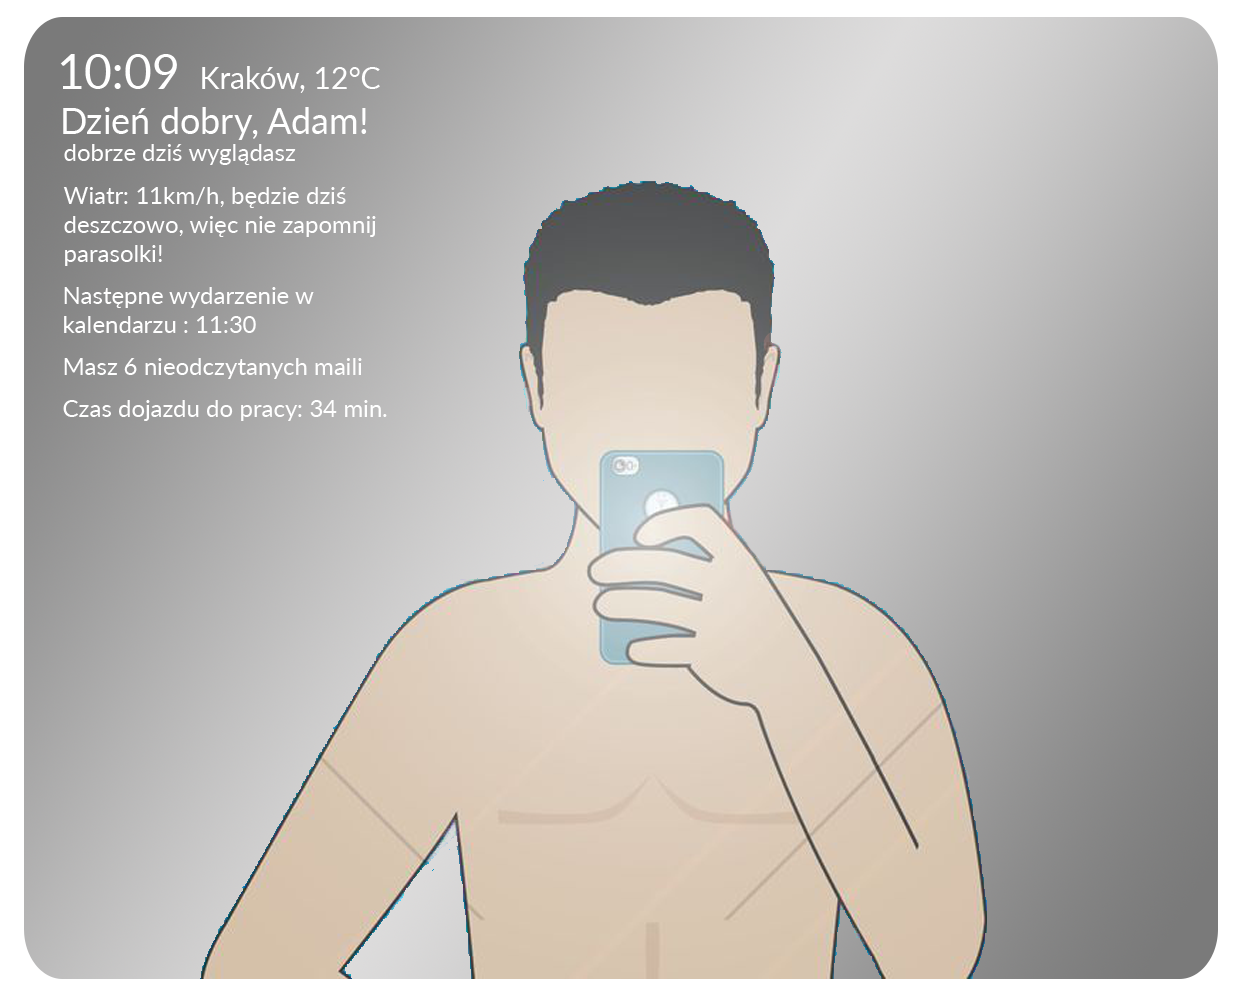
\includegraphics[width=0.6\textwidth,center]{mirror_on.png}
	\caption {Poglądowy rysunek lustra w stanie aktywnym}
	\label{lustro_on}
\end{figure}

\section{Możliwości personalizacji}
\begin{figure}[H]
	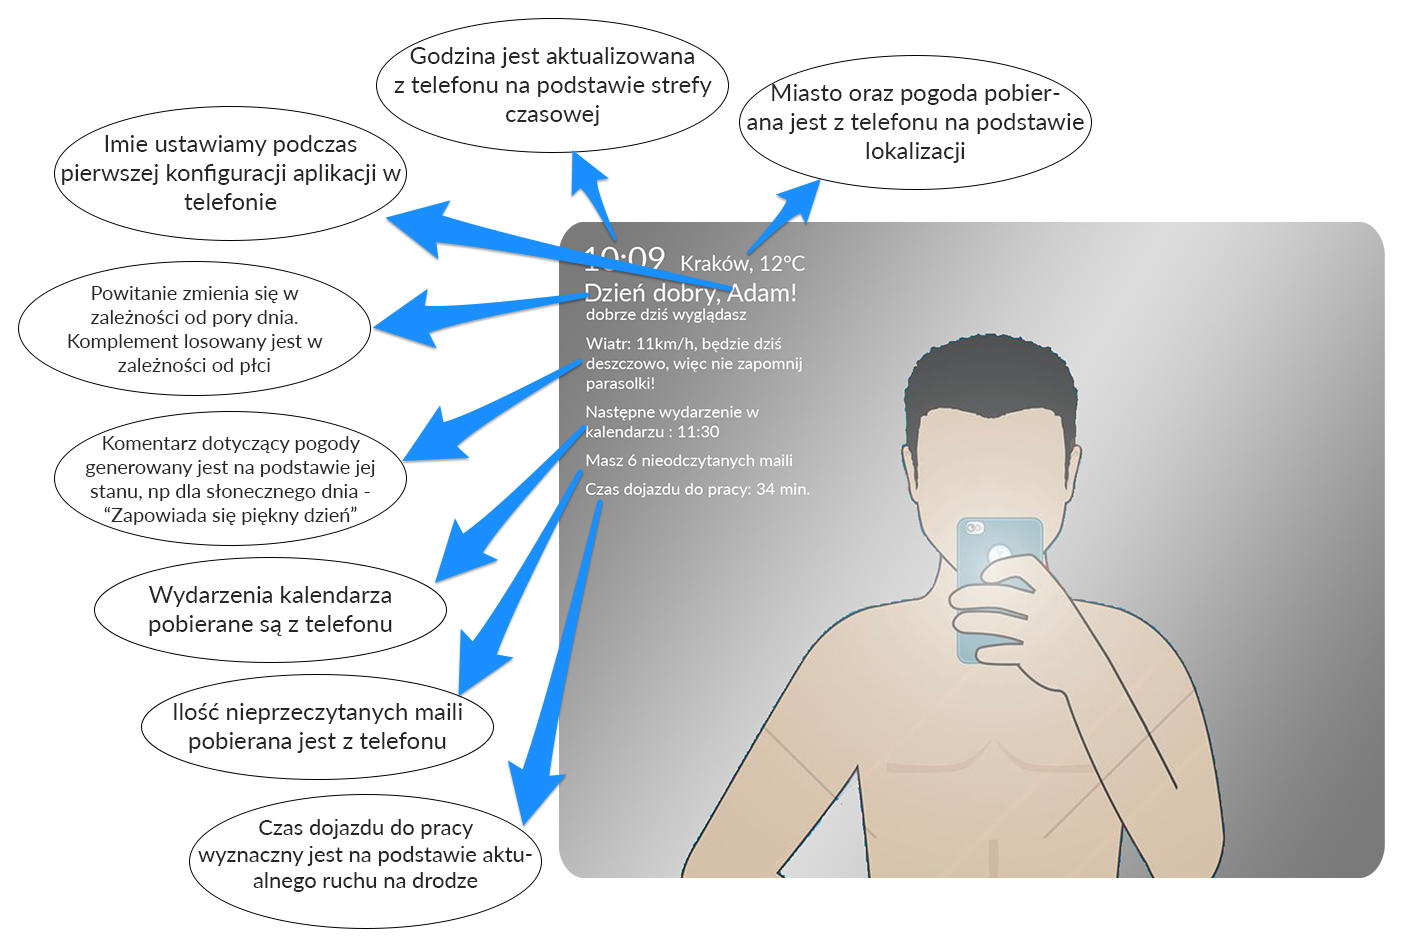
\includegraphics[width=0.9\textwidth,center]{dymki_kreski.png}
	\caption {Poglądowy rysunek możliwości personalizacji}
	\label{lustro_konf}
\end{figure}

\section{Opis aplikacji systemu wbudowanego nRF52}

\subsection{Włączenie urządzenia}
Urządzenie po uruchomieniu inicjalizuje wszystkie niezbędne usługi: timery, stos BLE, serwisy oraz obsługę wyświetlacza. Dalej rozpoczyna się rozgłaszanie (pod nazwą ,,nRF\_Reflekto'') i urządzenie pozostaje w stanie oczekiwania aż do wyłączenia zasilania. 

\subsection{Zasilanie}
Ze względu na użycie wyświetlacza TFT, wymagane jest zasilanie przez zasilacz zewnętrzny bądź port USB (bateria pastylkowa nie pokrywa zapotrzebowania na prąd). Szacowany pobór energii w stanie aktywnym wynosi 400mW. W stanie nieaktywnym pobór energii przez wyświetlacz może zostać zredukowany do zera (sterowanie PWM), jednakże wymaga to fizycznej ingerencji w płytkę wyświetlacza. W związku z tym zdecydowano o pozostawieniu przez cały czas aktywnego zegara, jako jedynej zawsze aktualnej informacji.

\subsection{Sposób rozgłaszania}
Do urządzenia w tym samym czasie może być podłączony jeden smartfon, ale z punktu widzenia użytkownika z lustra może korzystać kilka osób jednocześnie. Zostało to osiągnięte poprzez wprowadzenie 4-sekundowych slotów czasowych w przesyłaniu danych przez każdy smartfon. Wstępnie moc rozgłaszania została obniżona o 40dB (potrzebna jest późniejsza kalibracja w docelowym urządzeniu). Dzięki temu oszczędzana jest bateria w smartfonie jak i lustrze -- dane przesyłane są jak tylko lustro zostanie wykryte przez smartfona i nie jest wymagane ciągła aktywność w tle z urządzeniem.

Układ rozgłasza się pod wcześniej zdefiniowaną nazwą z dwoma servisami. Pierwszy posiada UUID ,,this is reflekto'' zapisane w systemie szesnastkowym (w celu unikalnej identyfikacji):
\begin{lstlisting}
	74686973-2069-7320-7265-666C656b746F
\end{lstlisting}
Drugi to ustandaryzowana usługa czasu o UUID  0x1805 zaimplementowana w urządzeniu.

\subsection{Zaimplementowane servisy}
W układzie zostały zaimplementowne cztery servisy \textit{Bluetooth Low Energy} których struktura i adresy są następujące:
\begin{itemize}
	\item 0x1805 -- Usługa aktualnego czasu
	\subitem 0x2A2B -- read/write -- czas w systemie unixowym
	\item 0x0010 -- Usługa pogodowa
	\subitem 0x0011 -- aktualne miasto, temperatura i ikona pogody
	\subitem 0x0012 -- aktualna prędkość wiatru
	\subitem 0x0013 -- porada pogodowa
	\item 0x0020 -- Usługa osobistych informacji
	\subitem 0x0021 -- następne wydarzenie z kalendarza
	\subitem 0x0022 -- informacja o nieodczytanych mailach
	\subitem 0x0023 -- prognozowany czas dojazdu do pracy
	\subitem 0x0024 -- imię użytkownika
	\subitem 0x0025 -- powitanie użytkownika
	\subitem 0x0026 -- komplement
	\item  0xDEAD -- Usługa konfiguracyjna
	\subitem 0xBEEF -- zapis informacji konfiguracyjnych
\end{itemize}
\subsection{Obsługa odbieranych danych}

Każda z wyświetlanych informacji przechowywana jest jako struktura zawierająca:
\begin{itemize}
	\item łańcuch znaków o ustalonej wcześniej długości (80 znaków)
	\item licznik ilości zapisanych znaków
	\item flagę mówiącą czy odbiór danych dla tego typu informacji został zakończony (czy jest możliwość poprawnego wyświetlenia całej informacji)
	\item flagę informującą czy informacja zmieniła się od ostatnio otrzymanej (czy jest konieczność jej ponownego wyświetlenia)
\end{itemize}

Z racji narzuconego limitu wielkości jednego pakietu \textit{BLE} do 20 bajtów, konieczne jest sklejanie poszczególnych paczek do jednego ciągu znaków. W tym celu skorzystano ze znaków \textit{ASCII}  oznaczonych jako \textit{STX -- Start of text} i \textit{ETX -- End of text}, które przedstawiają się formacie dziesiętnym jako cyfry $2$ i $3$.

W momencie otrzymania zapisu na jedną z charakterystyk obsługujących dane tekstowe, event przekazywany jest do funkcji łączącej dane. W przypadku otrzymania pakietu zaczynającego się od \textit{STX}, flagi oraz licznik znaków są zerowane i następuje zapis do łańcucha znaków. Porównywany jest otrzymany łańcuch z tym zapisanym poprzednio, dzięki temu wiadomo czy konieczne jest ponowne wyświetlenie danych. Odbiór kończy się w przypadku otrzymania znaku \textit{ETX} (na dowolnym miejscu). Ustawiana jest wtedy flaga zakończenia.

Przykładowo porada pogodowa ,,It will rain till tomorrow morning'' zostanie podzielona w następujący sposób:
\begin{enumerate}
	\item \textit{STX}It will rain till t
	\item omorrow morning\textit{ETX}
\end{enumerate}

Wielodniowe testy nie wykazały żadnych błędów przy stosowaniu powyższej metody transmisji i obsługi danych.

\subsection{Zabezpieczenia i charakterystyka konfiguracyjna}
Przy podłączeniu dowolnego urządzenia uruchamiany jest timer, który zezwala na pozostanie połączonym maksymalnie przez dwie sekundy. W praktyce pozwala to jedynie na odkrycie struktury urządzenia. W przypadku nie wpisania ustalonego hasła na charakterystykę konfiguracyjną, lub wpisaniu jakichkolwiek danych do systemu lustra przed podaniem go, połączenie zostaje natychmiast zerwane. Wpisanie hasła zatrzymuje timer i powoduje oczekiwanie na dane (np. w przypadku dłuższego niż zwykle pobierania danych z API).

Ze względu na optymalizację poboru energii smartfona, wykorzystywane jest specjalne hasło pozwalające na natychmiastowe rozłączenie z urządzeniem z ominięciem ograniczeń systemowych.

\subsection{Umieszczanie informacji na wyświetlaczu}
Ze względu na rodzaj wyświetlacza oraz użytą komunikację do przesyłu danych po \textit{SPI}, dostęp do wyświetlacza odbywa się pixel po pixelu. By zachować możliwość wybiórczego umieszczania i czyszczenia informacji, wyświetlacz został podzielony na sekcje:
\begin{itemize}
	\item Sekcja Czasu -- odświeżana selektywnie (sekundy co sekundę, minuty i godziny co 60 sekund, data w momencie zmiany dnia tygodnia)
	\item Sekcja Pogody -- odświeżana pojedynczo w przypadku zmiany otrzymanych danych, obejmuje zbiór 10 ikon pogodowych drukowanych pixel po pixelu, aktualne miasto, temperaturę, wiatr i poradę pogodową
	\item Sekcja Powitania i Komplementu -- odświeżana co 4 sekundy w przypadku obecności kilku użytkowników jednocześnie
	\item Sekcje e-mail, czasu dojazdu i kalendarza -- odświeżane w przypadku zmiany	
\end{itemize}

Wyświetlacz jest czyszczony w całości 30 sekund po rozłączeniu się ostatniego użytkownika. Odświeżanie zegara pozostaje wtedy bez zmian. Wygląd wyświetlacza przedstawia rysunek \ref{nrf_interface}.

\begin{figure}[H]
	\includegraphics[width=0.7\textwidth,center]{nrf_interface}
	\caption {Interfejs lustra}
	\label{nrf_interface}
\end{figure}

\section{Opis aplikacji systemu iOS (stan na 9 kwietnia 2017)}

Aplikacja mobilna po uruchomieniu automatycznie rozpoznaje lokalizację użytkownika z dokładnością ok. 3km oraz próbuje nawiązać połączenie bluetooth z modułem lustra. Aktualny wygląd aplikacji pokazany jest obrazie (Rys. \ref{ios_main_screen})

\begin{figure}[H]
	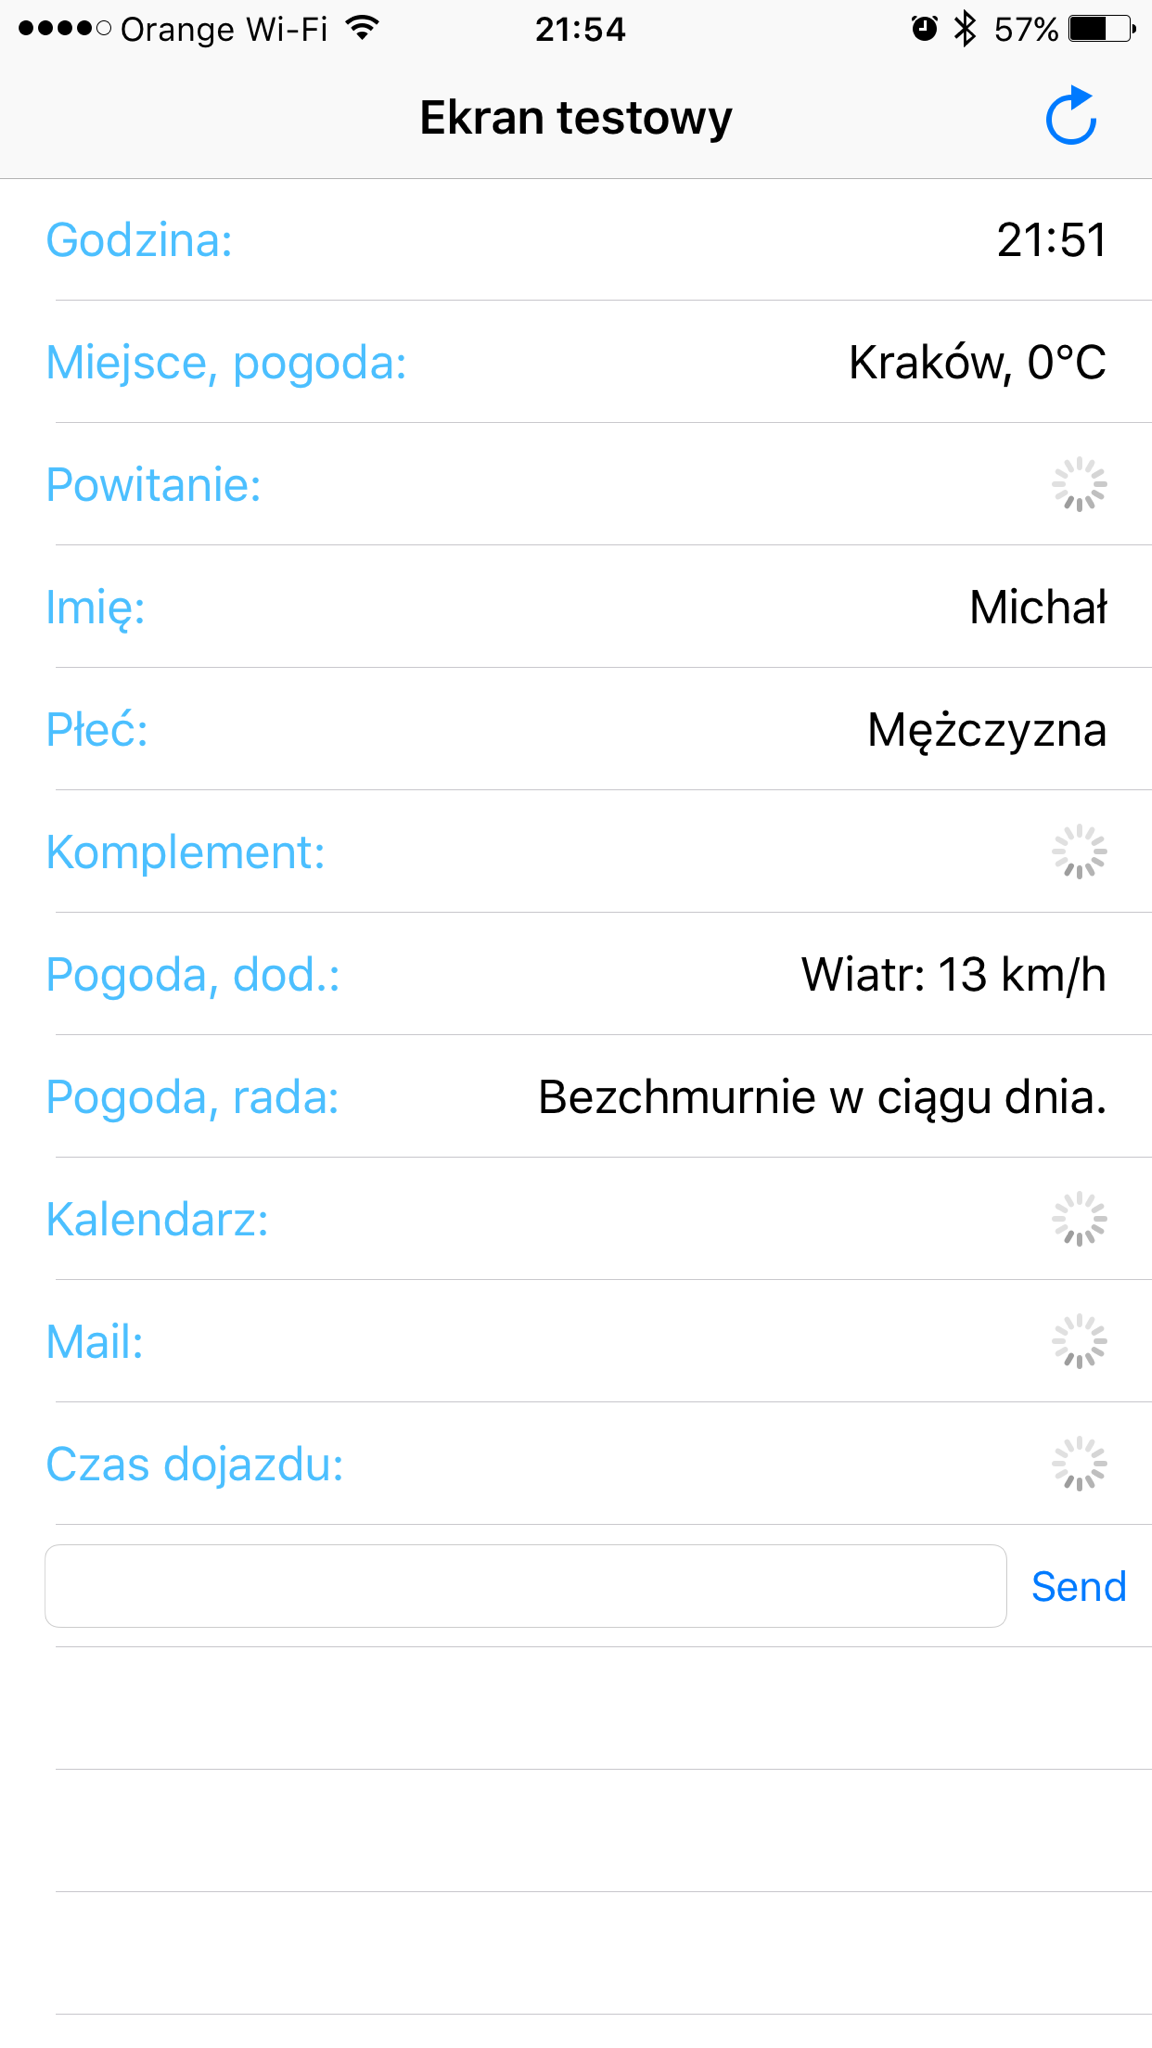
\includegraphics[width=0.4\textwidth,center]{ios_main_scrren.png}
	\caption {Aktualny wygląd aplikacji}
	\label{ios_main_screen}
\end{figure}

\subsection{Pobierane dane i sposób ich pobrania}
Aplikacja pobiera dane asynchronicznie, komórki z danymi w aplikacji uzupełniają się od razu po pobraniu poszczególnej danej. Nie trzeba czekać na zaktualizowanie interfejsu aż do momentu pobrania każdego elementu. Poniżej opis pobieranych danych oraz w przypadku bardziej złożonych informacji sposób ich pozyskania.

\begin{itemize}
	\item Godzina
	\item Miejsce, pogoda -- na podstawie wyznaczonej lokalizacji telefon wysyła zapytanie do Dark Sky API podając w parametrze m. in. długość oraz szerokość geograficzną. Otrzymany w odpowiedzi JSON parsowany jest na obiekt, z którego później wybierana jest temperatura. Miejsce wyznaczone jest również na podstawie szerokości i długości geograficznej używając wbudowanego  API Apple Maps.
	\item Imię -- imię użytkownika rozpoznawane jest automatycznie na podstawie nazwy urządzenia. Domyślnie ustawiona nazwa to np. ,,Michal's iPhone'' dla języka angielskiego lub ,,iPhone(Michał)'' dla języka polskiego. W przypadku innych wersji językowych nazwa urządzenia może być inna, więc metoda wykrywająca imię może nie zadziałać. Imię, które wykryjemy będzie jedynie propozycją podczas metody konfiguracji, jeśli użytkownik stwierdzi, że nie jest ono zgodne z prawdą będzie mógł je ręcznie wpisać.
	\item Płeć -- wyznaczana jest na podstawie ostatniej litery imienia, również będzie możliwa jej zmiana podczas procesu konfiguracji.
	\item Pogoda, dod. -- pobierana z Dark Sky API
	\item Pogoda, rada -- pobierana z Dark Sky API
\end{itemize}

\subsection{Sposób działania}
Po dotknięciu w poszczególną komórkę zostaje wygenerowany \textit{string} z dodanymi na początku dwoma bajtami, które pozwalają systemowi wbudowanemu zidentyfikować rodzaj informacji, która jest mu wysyłana. Po stworzeniu odpowiednich danych następuje próba wysłania informacji. Wykonywana jest na osobnym wątku, aby nie blokować interfejsu użytkownika.

W dolnej części interfejsu zostało dodane pole tekstowe ułatwiające proces przygotowania systemu wbudowanego. Można dzięki niemu wpisać dowolną informację, w jego przypadku nie są dodawane dodatkowe dwa bajty na początku.

\subsection{Planowany rozwój}

Aplikacja zostanie rozbudowana o proces konfiguracji, który użytkownik będzie musiał przejść tylko za pierwszym razem. Następne uruchomienia nie będą już wymagane, aplikacja będzie działać w tle i na podstawie skanera bluetooth uruchamiać się w pobliżu lustra. Dane będą dzielone na paczki i wysyłane do modułu bluetooth lustra.

Zostaną dodane kolejne dane pobierane z urządzenia, takie jak komplement generowany na podstawie płci lub informacje o nadchodzących wydarzeniach w kalendarzu.

Dodatkowo aplikacja zostanie przepisana, tak aby używała biblioteki RxSwift, która umożliwia pisanie kodu w sposób reaktywny i funkcjonalny. Do niektórych funkcji dodane zostaną również testy jednostkowe, oraz jeśli czas na to pozwoli integracja z systemem Travis w celu zastosowania continous integration.
	
	
\section{Podsumowanie}
	Projekt rozwijany jest z użyciem systemu kontroli wersji GitHub. Aktualne postępy dosępne są pod adresem: \url{https://github.com/Solstico}
	
	
	
	
	
	
\end{document}